\section{Suivi de la main dans une séquence d’images}
\subsection{Présentation de la méthode}

Les images du groupe 2, qui constituent une succession d’images, ne peuvent être traitées de la même manière que celles des deux autres groupes. En effet, notre méthode de segmentation telle qu’elle est conçue est idéale sur des images dans lesquelles la main est en avant-plan, ce qui n’est pas le cas sur l’ensemble d’images de ce groupe.
	Nous avons donc développé une méthode de traitement spéciale pour ce groupe, effectuant un suivi de la main dans l’image. L’idée générale de notre méthode est de suivre la main d’une image à l’autre afin de seuiller et ne garder uniquement la partie de l’image qui contient la main. Un tel algorithme pourrait être utilisé pour réaliser du suivi de main dans une séquence d’images quelconque, indépendamment de la reconnaissance. Notre méthode nécessite cependant de bénéficier à la base d’une image propre sur laquelle il est possible de réaliser une segmentation idéale.
	L’algorithme de suivi de la main est basé sur l’opérateur de Harris. Il permet d’effectuer un seuillage localisé sur la main d’une image à l’autre. Afin de localiser la main, on part à la base d’une image seuillée et on calcule la boîte englobante de la main. Cette même boîte englobante est utilisée sur l’image suivante de sorte que l’on obtienne deux fenêtres d’intérêt pour chaque image, partant du postulat que d’une image à l’autre, le mouvement de la main est minime. L’opérateur de Harris est alors appliqué sur chaque fenêtre (chaque main) de deux images consécutives. Après un appariement des points, on peut calculer un mouvement de la main par distance euclidienne de deux points appariés. Une nouvelle boîte sur laquelle on applique le mouvement est alors calculée et appliquée à la seconde image. Cette méthode est théoriquement efficace pour des mouvements latéraux de la main, mais lorsque celle-ci se rapproche ou s’éloigne de la caméra, un ajustement est nécessaire. C’est la raison pour laquelle la taille d’une boite englobante est élargie avant seuillage puis réadaptée.

L’algorithme développé peut être écrit comme suit :

\begin{itemize}
\item Segmentation de la main sur la première image.
\item Création de la boîte englobante (box).
\item Opérateur de Harris pour identifier les points d’intérêts.
\item Boucle : Pour chaque image consécutive
\begin{itemize}
\item Elargissement de la box.
\item Seuillage à l’intérieur de la box afin d’extraire la main.
\item Recadrage de la box si nécessaire.
\item Opérateur de Harris pour identifier les points d’intérêts.
\item Appariement des points de l’image seuillée et de la précédente.
\item Application du mouvement de la main sur le déplacement de la box.
\end{itemize}
\end{itemize}

\subsubsection{Segmentation de la main et extraction de la box}
Cette segmentation est « banale » et réutilise la méthode de segmentation générale basée sur l’algorithme de Fisher. A partir de l’image binarisée résultante, il est très simple de calculer les coordonnées de la boite englobante de la main extraite (\autoref{fig:boundingBox}).

\begin{figure}[htb!]
\centerline{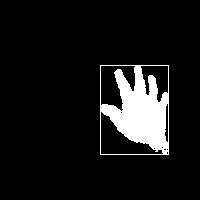
\includegraphics{boundingBox.jpg}}
\caption{Boîte englobante d'une main extraite.}
\label{fig:boundingBox}
\end{figure}

\subsubsection{Opérateur de Harris}
Dans la seconde étape importante, l’opérateur de Harris a été utilisé afin d’extraire les points d’intérêt de l’image seuillée. Ces points d’intérêt auraient pu être calculés sur l’image source, mais d’une image à l’autre, l’expérience a prouvé qu’aucuns points ne correspondaient, ce qui s'avérait problématique pour réaliser l’appariement d’une image à l’autre et détecter un mouvement. Sur l’image suivante, on observe les contours de la main ainsi que les points d’intérêt en blanc (\autoref{fig:harris}).

\begin{figure}[htb!]
\centerline{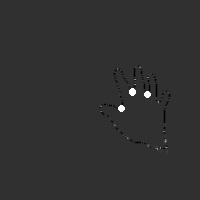
\includegraphics{harris.jpg}}
\caption{Points d'intérêts de la main par l'opérateur de Harris.}
\label{fig:harris}
\end{figure}

Pour chaque image consécutive :

\subsubsection{Seuillage sur la boite englobante}

Afin de préparer le terrain à l’opérateur de Harris, il est nécessaire de seuiller chaque image. L’identification du seuil est l’étape de l’algorithme qui présente le plus de problèmes et également celle qui est le plus à même d’être améliorée. Explications :
Selon l’image de la séquence qui est traitée, en partant du principe que la fenêtre est toujours centrée sur la main, il est évident que le contraste sera plus ou moins intense, que la profondeur de la main sera plus ou moins élevée, et donc que l’histogramme de cette main sera toujours différent d’une image à l’autre. La méthode de seuillage utilisée doit donc ici être particulièrement bien choisie si l’on veut que qu’elle fonctionne pour toutes les images d’une séquence.

Exemple de deux histogrammes selon une luminosité et un contraste différent : (\autoref{fig:histoLumin}).

\begin{figure}[htb!]
\centerline{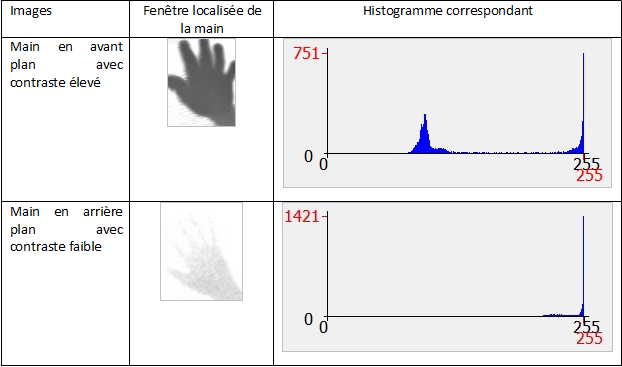
\includegraphics{table4.png}}
\caption{Histogrammes selon la luminosité et le contraste.}
\label{fig:histoLumin}
\end{figure}

Comme l’atteste le tableau ci-dessus (\autoref{fig:histoLumin}), nous avons affaire à des histogrammes bimodaux, même si c’est moins prononcé dans le second exemple de la main claire(en raison du nombre très élevé de valeurs de blanc). Il est cependant possible que l’histogramme ne suive pas le même schéma  et notamment que le deuxième mode ne soit pas 255 par exemple si on objet se trouve derrière la main ou si la main est devant le corps.
	La technique utilisée consiste à couper l’histogramme en deux parties via sa médiane (non pas sa moyenne). On recherche ensuite le mode sur le premier sous histogramme qui représente le niveau de gris le plus présent dans la main. On retient pour valeur de seuil un niveau de gris un peu plus élevé que le mode afin de seuiller la majeure partie de la main.

\[
Thresh = mode + n
\]
	Ca paramètre $n$ égal à 10 doit varier selon le contraste de la main. En effet, ce paramètre dépend de l’étendue de la première cloche de l’histogramme représentant le contraste de la main. Un faible contraste demandera une valeur faible tandis qu’un grand contraste demandera une valeur plus élevée. Tout l’enjeu ici est de seuiller correctement la main. Si le seuillage est trop faible ou trop élevé la binarisation donnera une image intraitable par le système de reconnaissance.

\subsubsection{Harris + Appariement des points de deux images seuillées}

Une fois le seuillage et la segmentation effectués, il est important de détecter le mouvement de lamain afin d’obtenir une nouvelle box pour cette seconde image. Si l’on se contentait de conserver l’ancienne box dont on s’est servi pour segmenter la nouvelle image, on pourrait d’une image à l’autre perdre de l’information dans la mesure où la main se déplace.

	Solution développée : On applique l’opérateur de Harris sur la nouvelle image seuillée afin de réaliser l’appariement avec l’image précédente, le but étant d’identifier le mouvement, déplacement des points d’intérêt.

	Une première solution a été implémentée afin d’apparier les points. D’une image à l’autre, les points d’intérêt étaient rattachés dans la mesure où leur distance euclidienne (de leurs coordonnées spatiales) était minimale. Cette méthode présentait le désavantage de chercher à minimiser le mouvement d’une image à une autre, ce qui ne correspondant pas forcément à la réalité.

	Une autre méthode de mise en corrélation a été développée et présente des résultats bien plus satisfaisants : SAD ( Sum of Absoute Differences )

	Pour chaque point d’intérêt, on calcule la mesure de similarité entre une fenêtre de taille 5 (paramètre variable) et la fenêtre du point d’intérêt d’une autre image : 

\[
\sum_{(u,v) \in W} |I_1(u,v) - I_2(u,v)|
\]

Considérant : $W$ la fenêtre d’encadrement d’un point d’intérêt.

La mesure de similarité est calculée sur l’image source et non l’image seuillée pour de meilleurs résultats. Une fois la valeur de similarité calculée entre chaque point d’intérêt des deux images, il faut les rattacher. Pour cela, on les rattache par leurs valeurs minimales. Un test est effectué sur la distance euclidienne entre les deux points afin d’éviter de rattacher des points trop éloignés. Cette étape évite de générer des outliers qu’il faudrait alors éliminer. Un point ne peut être apparié deux fois.
Exemple d’appariement pour deux images consécutives : (\autoref{fig:appariement}).

\begin{figure}[htb!]
\centerline{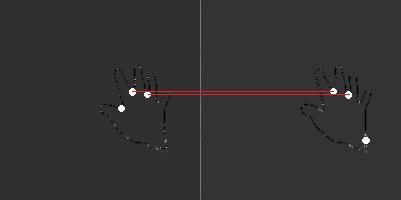
\includegraphics{appariement.jpg}}
\caption{Appariement pour deux images successives.}
\label{fig:appariement}
\end{figure}

La mise en correspondance des points permet d’obtenir un vecteur de translation $(a,b)$ pour chaque couple de points mis en corrélation. On peut alors obtenir un vecteur de translation moyen d’une image à l’autre : $(A,B)$.

\subsubsection{Déplacement de la box}

Une fois obtenue l’estimation d’un mouvement d’une image à l’autre, on peut alors appliquer le vecteur de translation aux coordonnées de la boite englobante sur la seconde image. Afin d’avoir un encadrement correct de la main. Ainsi, même si l’on perd un peu d’information sur le seuillage appliqué à la boite englobante d’une ancienne image, on le corrige grâce au mouvement obtenue par cette méthode, ce qui nous permet de conserver un encadrement correct de la main.

\subsubsection{Redimensionnement de la boîte}

Il y a un dernier point qui pose cependant problème et auquel nous avons du répondre : Lorsque la main est en mouvement, elle peut s’approcher ou s’éloigner de la caméra, ce qui est l’enjeu principal de la séquence d’images. De ce fait naît une problématique : 
	Sans considérer le seuillage de la main, celle-ci s’agrandit ou se rétrécit, et la taille de la boite englobante doit donc être modifiée en conséquence.

Solution envisagée:
\begin{itemize}
\item A chaque boucle (traitement d’une nouvelle image), la boite est élargie d’un pixel dans toutes les directions avant le seuillage.
\item La boite est redimensionnée si nécessaire après seuillage et segmentation de l’image. 
\end{itemize}

\subsection{Analyse des résultats}
Si la méthode générale développée et expliquée ci-dessus ne donne que des résultats moyennement satisfaisants, elle en donne tout de même puisque nous arrivons à effectuer un suivi de la main, au moins un temps. 
	On remarque que le suivi de la main dépend énormément du type de seuillage effectué. De nombreux tests donnant des séquences de résultats différents ont été effectués afin de développer une méthode de seuillage la plus efficace possible. Actuellement, la méthode de découpage d’histogrammes donne les « meilleurs » résultats, ou permet tout du moins de se focaliser sur la main, même si celle-ci est très rapidement mal seuillée et que la boite englobante n’englobe pas toute la main. (cf vidéo methode2\_0002.wmv).
	Une autre méthode de seuillage a été développée et présente des résultats différents : (cf vidéo : methode1\_0001.wmv). Cette méthode basique consiste à prendre le Xème niveau de gris non nul de la fenêtre encadrant la main. Elle présente un résultat différent puisqu’il est également efficace au début et rencontre une difficulté lorsque le poignet apparaît nettement dans l’image.

La raison pour laquelle ces deux méthodes ne fonctionnent pas convenablement est double :

Tout d’abord, le seuillage local n’est pas optimal car pas très intelligent. Compte tenu de l’impact du seuillage sur la qualité de la segmentation, une première amélioration de la détection de la main non négligeable consisterait à parfaire ce seuillage.
\begin{itemize}
\item Des tests ont été tentés à l’aide de l’algorithme de Fisher, mais en raison de difficultés techniques et de manque de temps, nous n’avons pu approfondir cette méthode qui devrait néanmoins pouvoir donner des résultats satisfaisants, découpant un histogramme en N classes.
\item Une segmentation par approche régionale (quadtree, graphes, …) pourrait être tentée et peut-être apportée des résultats corrects.
\end{itemize}

La seconde partie du problème réside dans l’adaptation de la box et notamment dans la phase d’agrandissement. Dans la séquence d’images étudiée, lorsque la main passe en arrière plan, le poignet se trouve confondu avec la main et est donc considéré comme en faisant partie (Méthode 1). A l’inverse, avec la seconde méthode de seuillage, la box se rétrécit pour n’encadrer que la paume de la main.

On comprend donc que l’adaptation de la box, si elle est indispensable va dépendre de la méthode de seuillage utilisée et donner une segmentation complètement différente suivant les techniques.
Une évolution du programme est donc de trouver le seuillage adapté à chaque type d’image.

\subsection{Améliorations possibles}
\begin{itemize}
\item Développement et test de nouvelles méthodes de seuillage.
\item Développer d’autres méthodes de corrélation pour Harris afin d’affiner la détection de mouvement.
\item Dans la suivi de mouvement, lorsque l’on traite deux images, une fois la nouvelle boîte englobante calculée pour la deuxième image, il serait envisageable de resegmenter cette image afin d’être sur de ne pas avoir perdu d’information. Cela devrait théoriquement éviter d’avoir parfois des mains rognées et donc améliorer la reconnaissance ensuite.
\end{itemize}
